% Template ripped from:
% http://www.cs.technion.ac.il/~yogi/Courses/CS-Scientific-Writing/examples/simple/simple.htm

\title{Differential Privacy with Dependent Types}
\author{
        Casper Holmgreen \\
        Department of Computer Science\\
        DIKU - Datalogisk Institut, K\o benhavns Universitet\\
        \and
        Knut Liest\o l\\
        Department of Computer Science\\
        DIKU - Datalogisk Institut, K\o benhavns Universitet\\
}
\date{\today}

\documentclass[12pt]{article}

\usepackage{graphicx}
\usepackage{listings}
\usepackage{amsfonts,amsthm,amsmath}

\newtheorem{defn}{Definition}[section]

\begin{document}
\maketitle

\lstset{language=Haskell,basicstyle=\footnotesize,frame=single,
        numbers=left}

\begin{abstract}
This is the paper's abstract \ldots
\end{abstract}

\section{Introduction}\label{sec:introduction}

% \subsection{Motivation/Overview}

With each passing day, more and more of our personal information is being collected, cataloged and analyzed by an ever increasing number of interested parties.
Their interests can range from targeted advertising to malicious and potentially illegal actions and everything in between.
As the producers of this data, we should be concerned with how it is being used.

For example, our medical records consist of very personal information which we expect to remain private.
Some countries even require legal privacy guarantees for systems maintaining sensitive information, e.g, the Health Insurance Portability and Acountability Act (HIPAA) in the USA.
The availability of an entire population's medical records would be a gold mine for medical researchers in need of statistical data.
And so we are faced with a classic balancing act: how do we balance individuals' privacy against the usefulness of a dataset?

Differential privacy\cite{journals/cacm/Dwork11} is an emerging field aiming to answer this question.
The central concept in differential privacy is indistinguishability, i.e, a query against a dataset should return more-or-less the same result regardless of whether or not a particular individuals records were included in the data.
If the results are indistinguishable, then the records of that particular individual must be unidentifiable.

Many metrics and algorithms have been developed by the differential privacy community.
Each algorithm is typically bundled with a formal proof that it meets some constraints or has some privacy-related properties.
The burden of producing such a proof and implementing the described algorithm is typically manual, and therefore error-prone.

PINQ\cite{conf/sigmod/McSherry09} is a differential privacy framework that takes a different approach.
It is a SQL-like query DSL for the .NET languages which guarantees differential privacy by construction.
Users of PINQ are able to compose carefully implemented primitives to build computations which run against raw data but cannot break differential privacy guarantees.
A protected runtime-system rejects queries whose cost exceed the remaining privacy budget.

These cost vs. budget checks are made at runtime.
An analyst has no way of knowing whether a query will be accepted by the runtime-system unless they are manually tracking their budget.
Reed and Pierce\cite{conf/icfp/ReedP10} solve this by building a strongly-typed programming language which represents query costs in the types.
We aim to extend this idea by showing that a dependent type system is a natural fit for capturing differential privacy requirements.

Strongly-typed languages are capable of statically verifying programs for type-correctness, precluding many potential sources of runtime errors: ``well-typed programs can't go wrong''.
We extend this notion of being ``well-typed'' to include differential privacy metrics.
Just as PINQ is embedded in the .NET languages (particularly C\#), we plan to embed our implementation within the dependently-typed, functional programming language: Idris\footnote{http://idris-lang.org}.
This allows us to take advantage of Idris' parser and advanced type checker, as well as the many constant improvements being made to them by the open-source community.

Well-typed programs in our embedded language can't go wrong and also can't violate their privacy requirements.
Formal proofs for type-correct algorithms written in our language are unnecessary - the program itself is the proof.
Thus, all type-correct programs must respect expected privacy requirements.

\subsection{Contributions}

This paper describes an implementation of an embedded prototype language, [NAME], for describing differentially private computations.
Dependent type systems have come a long way since Martin-L\"of's original intuitionistic type theory.
We show that dependent types in a practical setting are a natural fit for describing concepts from differential privacy.

\paragraph{Outline}
The remainder of this article is organized as follows.
Section~\ref{sec:background} provides background and gives account of previous work.
Section~\ref{sec:implementation} describes our implementation.
We evaluate our implementation in Section~\ref{sec:evaluation}.
Section~\ref{sec:discussion} discusses the implementation and potential future work.
Finally, Section~\ref{sec:conclusions} gives the conclusions.

\section{Background}\label{sec:background}

This section provides light background information on differential privacy, dependent types, and relational algebra.

\subsection{Differential Privacy}\label{sec:differential_privacy}

In today's Big Data world, more and more of our data is being stored on servers belonging to others.
We are not the consumers of free online services, we are the product.
But regardless of whether we freely volunteered it, were legally compelled to share it, or just bought something online, we have a reasonable expectation to privacy of our data.

However, databases containing large amounts of personal data can be tremendously valuable for researchers looking into a variety of important questions.
For example, epidemiologists may be able to detect and prevent the spread of disease and doctors may be able to monitor and/or analyze the long-term health trends of a large population over time.
Big Data offers us huge potential for learning about ourselves, but most of these databases are held under lock and key.
How best to balance database utility against individual privacy is the question differential privacy aims to answer.

Many approaches have been devised for sharing data while respecting privacy.
One approach, which has made news headlines a few times by now, is to anonymize or otherwise ``fuzz'' a dataset before releasing it to the public.
However, it is increasingly evident that it is not possible to release a database accurate enough to be usable while still respecting privacy\cite{journals/cacm/Dwork11}.

Differential privacy aims to maximize database utility while minimizing the risk for all individuals contained within.
Traditionally, privacy research has focused on preventing a malicious attacker from learning anything about any given individual.
However, this has proved to be nearly impossible in the presence of auxiliary information. ((WHY))
% TODO: why?

Rather than trying to prove the impossibility of a privacy breach, differential privacy guarantees that a users participation in a database will only increase their risk of a privacy breach by some small amount.
This holds true regardless of how much auxiliary information a would-be attacker knows.

Analysts are able to run differentially private algorithms against raw data knowing that no individuals' privacy can be compromised.
Suddenly, many of the Big Data databases which would otherwise be off limits can be made available to researchers.
Each individuals participation in the database does not have a large effect on their privacy risk, so honest participation is almost a direct consequence.

\subsubsection{Function Sensitivity}
% TODO: give a better subsubsection name

One of the key metrics used in differential privacy, and in our type system, is function sensitivity.
Function sensitivity provides an upper bound on how much a function can magnify distances between inputs.

\begin{defn}\label{def:csens}
  A function, $f : \mathbb{R} \rightarrow \mathbb{R}$, is $c$-sensitive if
  $\forall x,y.d(f(x),f(y)) \le c \times d(x,y)$.
\end{defn}

As an example, take the Euclidian distance function, $d_\mathbb{R}(x,y) = |x - y|$, for $d$.
Clearly, the function $f_1(x)=x$ cannot magnify distances at all.
For any two real numbers, their difference will equal the difference between them after applying $f_1$.

\[
  \forall x,y.d_\mathbb{R}(f_1(x),f_1(y)) = d_\mathbb{R}(x,y)
\]

We say $f_1$ is 1-sensitive.
Another example of a 1-sensitive function is $f_2(x) = x/2$.

By choosing a different distance function, function sensitivity can be extended to be applicable to almost anything.
Differential privacy is primarily concerned with databases, so we choose an appropriate distance function over $\mathbb{D}$.
Given two databases, $D_1, D_2 \in \mathbb{D}$, we define the distance between them to be the length of the symmetric difference of their elements (or rows).
That is, $d_\mathbb{D}(D_1,D_2) = |D_1 \oplus D_2|$.

We define a special case when two databases differ by exactly one row (i.e. $d_\mathbb{D}(D_1,D_2)=1$), which we denote by $D_1 \sim D_2$.
This is a common-case in the differential privacy literature because we are concerned with the inclusion of any particular individual's data in the database.
One of the databases contains that individual's data; the other is the same database with exactly that row removed.

\subsubsection{Indistinguishability}

One of the key concepts driving differential privacy research is that of indistinguishability.
The idea is simple: if an attacker, based on the output from a query, is unable to determine whether your data was even included in the database, then he can't deduce much about your data from the database.
We turn to randomness to achieve this kind of property.

Consider a randomized function, $f_r(x)$.
Assume that we have two variables, $x, y \in Domain(f_r)$.
If the probability of $f_r$'s output being in $S \subseteq Codomain(f_r)$ is almost the same regardless of whether $f_r$ was applied to $x$ or $y$, then it is nearly impossible to determine which input was used.

\[
  Pr[f_r(x)\in S] \qquad\approx\qquad  Pr[f_r(y)\in S]
\]

This is the core idea behind indistinguishability.
Now consider a randomized query, or mechanism, $\mathcal{M}(D) : \mathbb{D} \rightarrow \mathbb{R}$.
We say that such a query is $\epsilon$-differentially-private if the inclusion of your data affects your privacy risk by at most $e^\epsilon$.

\begin{defn}\label{def:diffpriv}
  A randomized mechanism, $\mathcal{M}(D)$, is $\epsilon$-differentially-private if, for all databases $D_1 \sim D_2$, and all $S \in Codomain(M)$,
  $Pr[\mathcal{M}(D_1)\in S] \le e^\epsilon \times Pr[\mathcal{M}(D_2)\in S]$.
\end{defn}

\begin{itemize}
  \item Quick talk about PINQ?
  \item Other stuff
\end{itemize}

\subsection{PINQ}\label{sec:pinq}

This section will provide an overview of PINQ, the language we used as model for our language. PINQ is a layer built on top of the query language LINQ, providing some differential privacy guarantees.

\subsubsection{Aggregations}

The only way to extract data from the underlying database in PINQ is by using the built-in aggregation functions. These aggregations are proven to be $\epsilon$-differentially private. $\epsilon$ is a precision parameter passed in with aggregation applications.

One of these aggregations is \texttt{count}, which counts the number of rows in the given query. In order to prove the sensitivity of this function we can use definition $\ref{def:csens}$. 
Let the distance function \texttt{d} be the Euclidean distance. Let the domain of \texttt{f} be two databases $D_1$ and $D_2$ where $D_1 \sim D_2$, representing a database with and without a particular individuals record. If we take the count of both these databases, we see that the Euclidean distance between the counts will always be 1, and thus count is a 1-sensitive function.

Following definition $\ref{def:diffpriv}$, we can make count $\epsilon$-differentially private by adding zero mean Laplacian noise with 1/$\epsilon$ standard deviation to the result (TODO: Why). We call this version of count \texttt{noisyCount}. $\epsilon$ is a parameter of all the noisy aggregations and represents the balance between precision and privacy.

Another aggregation we provide is average. Using the same approach, we find that the distance is dependent on the range of the type we are averaging. PINQ chooses to clamp the range between -1 and 1, which makes the function 1-sensitive. The consequence is that users have to pre-process the data by normalization before they use \texttt{noisyAverage}, which is the name of the average function with the added Laplacian noise as with count.

\subsubsection{Transformations}

Aggregations on their own are somewhat limited in their analytic power, but combined with transformations they become more powerful.
The raw data results produced from transformations can not be exposed to users, as this would leak large amounts of privacy, but can be used as input to the aggregations, providing more flexibility.

In PINQ, the sensitivity of a transformation is referred to as its stability. Proving the stability of a transformation is an application of definition \ref{def:csens} where \texttt{c} is the stability, \texttt{f} is of type  $D_1 \sim D_2 -> D$ and the distance function \texttt{d} is the symmetric difference.

Examples of 1-stable transformations are \texttt{select} and \texttt{where}. 

\texttt{select} is a projection and will return the same number of rows as the input, and thus removing a particular row in the input will remove exactly one row and affect no other row of the result.

\texttt{where} is a selection and will return a subset of the input rows. If we remove one of the input rows, the change in the result will be at most one row.

\texttt{groupBy} is an example of a 2-stable transformation. This is because removing one row of the input can potentially both remove a group and the member in this group, leading to a symmetric difference of 2.

For an aggregation applied to subsequent transformations the sensitivity is the stability of the transformations multiplied by $\epsilon$.

For example $\texttt{count} \circ \texttt{groupBy} \circ \texttt{groupBy}$ will be a $4\epsilon$-differentially private function.

\subsubsection{Budget}

For every data source in PINQ a global budget is user-defined. Whenever a successful aggregation has been performed, its sensitivity is subtracted from the budget.
If the privacy cost of the aggregation exceeds the remaining budget, the aggregation request gets denied.


\subsection{Dependent Types}

Type-systems have been a point of contention in the programming community for many, many years.
There is no doubt, however, that strong type-systems are able to preclude many different types of runtime errors.
In fact, a very good type system will allow the programmer to record their assumptions about a program with ease and allow the machine to check them.

The ``strength'' of a type-system can vary a lot.
Languages like C provide very little in the way of strong types: everything is assumed to be a number until explicitly told otherwise (e.g, in a call to \texttt{printf(..)}).
Others, like Java, provide strong static typing, but at the cost of requiring a lot of boilerplate code for type annotations.
Haskell is a strong, statically-typed programming language capable of providing compile-time guarantees and type inference, reducing boilerplate code considerably.

In this paper, we will be looking primarily at the Idris language\footnote{http://idris-lang.org}.
Idris is a dependently-typed language written in Haskell under very active development.
Syntactically, Idris looks a lot like Haskell - indeed, many of their syntactic design decisions were made based on Haskell's - but it is a very different language.

In particular, Idris has traded Haskell's type inference for dependent types.
Dependent types are types that can depend on values.
Most type systems allow types to be constructed from other types.

\begin{defn}
  A \textbf{concrete type} is a type with no type holes, i.e, it has type $\tau$. Examples include \texttt{Int}, \texttt{String}, \texttt{List Int}.
\end{defn}

\begin{defn}
  A \textbf{type constructor} is a function of the form
  $\mathcal{F} : \tau \rightarrow \tau$. Type constructors may include one or more type parameters (e.g, $\mathcal{F} : \tau \rightarrow \tau \rightarrow \tau$.
  Examples include \texttt{List a}, \texttt{StateT s m a}, and \texttt{Maybe a}.
\end{defn}

A simple example of a type constructor with arity 1 is $List : \tau \rightarrow \tau$.
$List$ is not a concrete type until we apply it to another (concrete) type (e.g, applying $List$ to $Int$ results in a $List\ Int : \tau$).

Dependent types relax the restriction on type parameters, allowing us to index types by values as well as types.
The arguments to type constructors as defined above do not have to be concrete types, but may now be values (of concrete types).

\begin{defn}
  A \textbf{dependent type constructor} is a function of the form
  $\mathcal{F} : (a : \tau) \rightarrow a \rightarrow \tau$, where we abuse notation to assume $\tau : \tau$.
  $Vect : \mathbb{N} \rightarrow \tau \rightarrow \tau$ is a common example of a dependent type constructor.
\end{defn}

The classic example of a dependent type is the $List$ indexed by length, commonly referred to as a ``vector''.

\begin{alignat*}{2}
  List &:                        &&\tau \rightarrow \tau \\
  Vect &: \mathbb{N} \rightarrow &&\tau \rightarrow \tau
\end{alignat*}


Examples of well-typed $Vect$s include $[1,2,3]\in Vect\ 3\ Int$ and $[]\in Vect\ 0\ String$, but not $[1,2]\in Vect\ 3\ Int$.

See Listing~\ref{lst:vect} for implementations of $List$ and $Vect$ in Idris.
Listing~\ref{lst:vect} also includes type annotations for \texttt{head} and \texttt{append}.
The $List$ \texttt{head} and \texttt{append} functions provide no formal guarantees about anything other than the return type.
What would happen if we took the \texttt{head} of an empty list?
What prevents us from writing a definition for \texttt{append} which ignores it's second argument and just returns the first argument?

The $Vect$ versions of the same functions rule out both of these possibilities.
It is impossible to take the \texttt{head} of an empty $Vect$, because an empty $Vect$ can never be passed to it.
The types do not match and the compiler will complain.
Additionally, the resulting vector of an \texttt{append} operation \textbf{must} be of length $n+m$.
Of course, there are many semantically incorrect ways of writing the definition for \texttt{append} while satisfying the length requirement, but the compiler will be able to prevent a large subset of incorrect implementations based on the length guarantee.

\begin{lstlisting}[caption=List and Vect,label={lst:vect}]
data Nat : Type where
  Z : Nat
  S : Nat -> Nat

data List : Type -> Type where
  Nil  : List a
  (::) : a -> List a -> List a

data Vect : Nat -> Type -> Type where
  Nil  : List Z a
  (::) : a -> List n a -> List (S n) a

head   : List a -> a
head   : Vect (S n) a -> a

append : List a -> List a -> List a
append : Vect n a -> Vect m a -> Vect (n+m) a
\end{lstlisting}

The usefulness of dependent types extends far beyond keeping track of $List$ lengths.
They have been used for writing type-safe resource management APIs, network protocol parsers, and much more\cite{conf/plpv/Brady11}.
We believe that dependent types are a natural fit for modelling differential privacy in a type-safe manner.

\subsubsection{Example: Sensitive functions with dependent types}

Function sensitivity composes according to simple arithmetic functions over values and dependent types allow us to index types by values.
Differential privacy can be recorded and enforced directly in dependent function type signatures.

Now we illustrate a simple example of using dependent types for capturing function sensitivity.
We want to be able to construct functions indexed by sensitivity and compose them.
Additionally, we want to write an application function which, given a sensitive function, maximum sensitivity, and input value, applies the function to it's input value if the function sensitivity does not exceed the given maximum sensitivity.

We name the sensitive function type \texttt{Private s a b}, where \texttt{s} represents the sensitivity (as a floating point value), and \texttt{a} and \texttt{b} represent the input and output types.
There is only one data constructor, \texttt{MkPrivate}, wrapping a native Idris function.
For now, we will model sensitivity as a floating-point value.
This is not necessarily the best choice, but it is sufficient for illustration purposes.
More on this later.

\begin{lstlisting}[caption="Sensitive functions in Idris"]
data Private : Float -> Type -> Type -> Type where
  MkPrivate  : (a -> b) -> Private s a b
\end{lstlisting}

Now we can make a few sensitive functions.
At this point, we must rely on the user providing accurate function sensitivities in the type annotations.

\begin{lstlisting}[caption="Simple examples of sensitive functions"]
foo : Private 1 Int Int
foo = MkPrivate (\x => x)

bar : Private 1 Float Float
bar = MkPrivate (\x => x / 2)
\end{lstlisting}

Suppose we want to compose \texttt{foo} and \texttt{bar}.
They are now wrapped behind a data constructor, so we can't just use Idris' native \texttt{(.)} operator.
Even if we could, we need to handle the merging of sensitivities.
We abstract the specific details away with an operator: \texttt{(.+.)} (but implement it as basic addition for illustrative purposes).
Given an implementation of \texttt{(.+.)}, we can implement function composition for \texttt{Private} computations.
(Also, note that Idris allows function name overloading as long as the correct instance can be determined uniquely from the types.)

\begin{lstlisting}[caption=Composing function sensitivity]
(.+.) : Float -> Float -> Float
(.+.) = (+)

(.) : Private s b c -> Private s' a b -> Private (s .+. s') a c
(.) (MkPrivate f) (MkPrivate g) = MkPrivate (f . g)
\end{lstlisting}

All that is missing now is function application.
The user will provide it with a private function, a maximum sensitivity, and an input value.
\texttt{apply} will require a proof that the sensitivity of the given function does not exceed the specified maximum sensitivity.
We use Idris' implicit, automatic proof search for this, so the user will not need to deal with it (unless they are trying to exceed the maximum sensitivity).

\begin{lstlisting}[caption="Private function application"]
  apply : Private s a b -> a -> (t:Float) -> {auto p : So (s <= t)} -> b
  apply (MkPrivate f) x _ = f x
\end{lstlisting}

Now we are able to apply \texttt{Private} functions to values if we do not exceed a specified maximum sensitivity.
The type-checker will reject any illegal function applications \textit{at compile-time}.

\begin{lstlisting}
apply (foo . bar) 1 1 -- does not type-check: 2 <= 1 not true
apply (foo . bar) 1 10 -- does type-check: 2 <= 10
\end{lstlisting}

\subsection{Relational Algebra}

The relational algebra describes semantics of relational datastores and queries over them.
There have been numerous attempts to formalize relational algebra in type systems %TODO : add citations. Include Henglein & Larsen? HaskellDB
, particularly in Haskell.
Oury and Swierstra demonstrate how dependent types can be used\cite{OurySwierstra08PowerOfPi}.
We arrived at the same result independently and like it very much.
% TODO : how to rewrite prev. sentence?

The benefit to focusing our research on the relational algebra is that our results are as general as the relational algebra.
Indeed, we demonstrate two different backends for our language.
Anything which can be described by the relational algebra can be made differentially private. % TODO : is this claim too bold?

An algebra describes a set of symbols and operations over the symbols.
For example, the set of all natural numbers, $\mathbb{N}$, with the operations $\{+,-\}$, is an algebra.

In the case of relational algebra, the symbols are relations, or, if we abuse our imaginations a little bit, tables.
There are five primitive operations as laid out by Codd\cite{codd70} and one rename operator:

\begin{itemize}
  \item $\sigma$ - selection
  \item $\pi$    - projection
  \item $\times$ - cartesian product
  \item $\cup$   - union
  \item $\cap$   - difference
  \item $\rho$   - rename
\end{itemize}

Union and difference only differ from Set union and difference in the addition of schema constraints.
The same is true of the cartesian product.

\begin{figure}[tb]
  \centering
  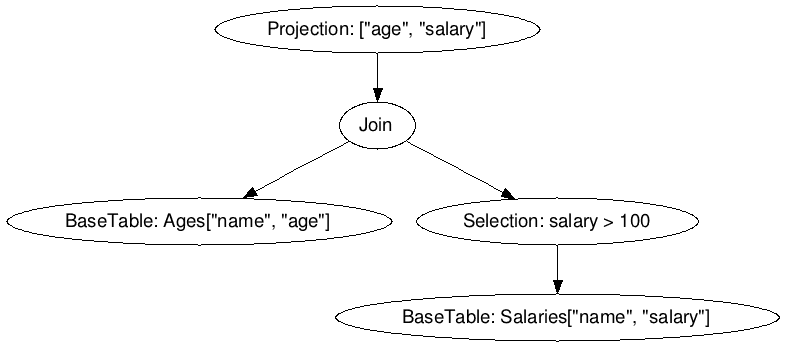
\includegraphics[width=\textwidth]{assets/relalg.jpg}
  \caption{Example of relational algebra}
  \label{fig:example_relalg}
\end{figure}

From these operators and armed with dependent types, we can now construct type-safe queries over relational data stores.
See Figure~\ref{fig:example_relalg} for a visual example.

\subsection{Related work}\label{sec:related_work}

\begin{itemize}
  \item PINQ
  \item (D)Fuzz
  \item Airavat
  \item \ldots
\end{itemize}

\section{Implementation}\label{sec:implementation}

Our implementation consists of two parts: a LINQ-like relational algebra and query engine, and a PINQ-like interface providing compositional differential privacy mechanisms.

\subsection{Power of Pi}\label{sec:power_of_pi}

How to best represent the relational algebra with static types has been an open research question for some time.
There are a variety of approaches offering different degrees of static guarantees.
Most have been limited by the power of the type systems they targetted.
In particular, the requirements on operations such as \texttt{product} pose problems for limited type systems.

Idris provides a rich, dependent-type system, which allows for much stronger guarantees.
In particular, we are capable of fully representing schemas, expressions, and transformations with dependent types.

A schema describes the structured format of a database table.
For example, a database table \texttt{people} may consist of two columns: \texttt{name} and \texttt{age}.
An \texttt{Attribute} is a pair consisting of name and type.
\texttt{age} is an attribute most likely represented by an unsigned integer.
A database \texttt{Schema} is then just a list of \texttt{Attribute}s.
See Listing~\ref{lst:schemas} for an example in Idris.
Note that we represent the database type using native Idris types.
% TODO : discuss why this is good.

\begin{lstlisting}[label={lst:schemas},caption=Representing schemas with dependent types]
data Attribute : Type where
  (:::) : String -> Type -> Attribute

Schema : Type
Schema = List Attribute

people : Schema
people = ["name":::String,"age":::Int]
\end{lstlisting}

Armed with a solid \texttt{Schema} representation, it is easy to symbolically represent an expression language.
Expressions will be necessary for some of the relational algebra operators.
Listing~\ref{lst:expr} shows an incomplete example.

\begin{lstlisting}[label={lst:expr},caption=Representing typed expressions]
data Expr : (s:Schema) -> (t:Type) -> Type where
  (^) : (s:Schema) -> (nm:String)
     -> { auto p : (map cast s) `ContainsKey` nm }
     -> Expr s (lookupType s p)
  (+) : Num t  => Expr s t -> Expr s t -> Expr s t
  (==): Eq t   => Expr s t -> Expr s t -> Expr s Bool
  Lit : Show t => (val:t) -> Expr s t
  PureFn : (a -> b) -> Expr s a -> Expr s b

fountain_of_youth : Expr people Int
fountain_of_youth = people^"age" + (-10)
\end{lstlisting}

Now, we have everything necessary to represent the relational algebra.
Listing~\ref{lst:query} shows our implementation.
\texttt{Disjoint s s'} is a proof that two schemas, \texttt{s} and \texttt{s'} are disjoint.
\texttt{projectedSchema} applies and filters the types of a projection.
Note that renaming is a general case of projection.
\texttt{Query} is a type family indexed by backend.
This allows us to generalize the relational algebra to in-memory Idris databases as well as SQL-based databases such as SQLite.

\begin{lstlisting}[label={lst:query},caption=Representing typed queries]
data Query : (b:Backend) -> (s:Schema) -> Type where
  Table   : TableType b s -> Query b s
  Union   : Query b s -> Query b s -> Query b s
  Diff    : Query b s -> Query b s -> Query b s
  Product : Query b s -> Query b s'
         -> { auto p : Disjoint s s' } -> Query b (s ++ s')
  Projection : (f:String -> Maybe String) -> Query b s
            -> Query b (projectedSchema f s)
  Select  : Expr s Bool -> Query b s -> Query b s
\end{lstlisting}

% TODO : show an example of a Query on peoplea

\subsection{PINQ}\label{sec:implementation:pinq}

This section will descibe our implementation of the differential privacy aspects of our language. We follow PINQ's model of building a differential privacy layer on top of a query language.

\subsubsection{PINQuery}\label{sec:pinq:pinquery}

\begin{lstlisting}[label={lst:pinquery},caption=PINQuery - wrapper around Query]
data PINQuery : Backend -> Schema -> Stability -> Type  where
  MkPINQuery : Query b s -> PINQuery b s c
\end{lstlisting}

\texttt{PINQuery} is a type that represents a query with stability, which is a concept mentioned in section $\ref{sec:pinq}$. 
The type has only one type constructor, taking a \texttt{Query} as an argument. The Query type is described in $\ref{sec:power_of_pi}$.

\begin{lstlisting}[label={lst:where},caption=Selection on PINQuery]
where' : PINQuery b s c -> Expr s Bool -> PINQuery b s c
where' (MkPINQuery q) e = MkPINQuery (Select e q)
\end{lstlisting}

The transformation functions on PINQueries are just calling the analog transformation of the Power of Pi query language on the encapsulated Query.
The interesting thing happens in their type signatures. 
As for \texttt{where'} in listing $\ref{lst:where}$, because it is a 1-sensitive function, it just copies the stability of the incoming PINQuery to the result.


\begin{lstlisting}[label={lst:groupBy},caption=groupBy]
groupBy : Eq k => Expr s k -> PINQuery b s c -> PINQuery b ["k":::k, "v"::: TableType b s] (c * 2)
groupBy e (MkPINQuery q) = MkPINQuery (GroupBy e q)
\end{lstlisting}

In listing $\ref{lst:groupBy}$ we can see \texttt{groupBy}, which has a more complex type signature.
Because we know that it has a stability of 2, we multiply the sensitivity of the incoming PINQuery by 2.

\begin{lstlisting}[label={lst:aggregation},caption=Aggregation type class]

||| Aggregation type class that keeps track of the sensitivity
class Aggregation (pinq : Schema -> Stability-> Type) where
    noisyCount : pinq s c -> (e:Epsilon) -> Private (c*e) Double
    noisyAverage : Expr s Double -> pinq s c -> (e:Epsilon) -> Private (c*e) Double
\end{lstlisting}

The aggregation functions' type signatures are captured in a type class shown in listing $\ref{lst:aggregation}$.
A type class is chosen in order to allow for different implementations of the evaluation function, i.e. native Idris execution, or compilation to a query language like SQL.


\section{Evaluation / Validation}\label{sec:evaluation}

\section{Discussion}\label{sec:discussion}

\subsection{Future work}\label{sec:future_work}

\begin{itemize}
  \item CSPRING
  \item Effects?
\end{itemize}

\section{Conclusions}\label{sec:conclusions}
We worked hard, and achieved very little.

\bibliographystyle{abbrv}
\bibliography{main}

\end{document}
